%% —-----------------------------------------------------------
%% sbcreviews-pt.tex
%% Template para SBC Reviews 
%% (https://journals-sol.sbc.org.br/index.php/reviews/) 
%% 
%% Esta versão do template para a SBC Reviews inclui algumas
%% modificações sobre o template original da REIC
%% (https://journals-sol.sbc.org.br/index.php/reic)
%%
%% Licença CC BY 4.0 (https://creativecommons.org/licenses/by/4.0/)
%% Sociedade Brasileira de Computação.

\documentclass[portuguese]{sbcreviews-2025}%
\usepackage[misc,geometry]{ifsym} 

%\usepackage{graphicx} % carregada dentro da classe
%\usepackage{fontspec} % carregada dentro da classe
%\usepackage{fontawesome} % carregada dentro da classe
%\usepackage{color} % carregada dentro da classe
%\usepackage{hyperref} % carregada dentro da classe

\usepackage{aas_macros}
\usepackage[bottom]{footmisc}

\usepackage{tabularray}
% O pacote tabularray torna o uso dos pacotes abaixo desnecessarios.
%\usepackage{supertabular}
%\usepackage{multicol}
%\usepackage{multirow}

\usepackage{afterpage}
\usepackage{url}
\usepackage{pifont}
\usepackage{caption}

\setcitestyle{square}

\definecolor{engtitle}{rgb}{0.5,0.5,0.5}
\definecolor{orcidlogo}{rgb}{0.37,0.48,0.13}
\definecolor{unilogo}{rgb}{0.16, 0.26, 0.58}
\definecolor{maillogo}{rgb}{0.58, 0.16, 0.26}
\definecolor{darkblue}{rgb}{0.0,0.0,0.0}
\hypersetup{colorlinks,breaklinks,
            linkcolor=darkblue,urlcolor=darkblue,
            anchorcolor=darkblue,citecolor=darkblue}
%\hypersetup{colorlinks,citecolor=blue,linkcolor=blue,urlcolor=blue}
% We disable hyperlinks by default with this line, to avoid the error "\pdfendlink ended up in different nesting level" while writing.

\jid{ROCS}
\jtitle{SBC Computing Reviews, 202X, XX:1}
\issn{2966-3938}
\doi{10.5753/rocs.202X.XXXXXX}
\copyrightstatement{Este trabalho está licenciado sob uma Licença Creative Commons Atribuição 4.0 Internacional}
\jyear{202X}

\category{Artigo completo}
\title[Template da SBC Reviews 2025 para artigos em português]{Uma Revisão Bibliográfica sobre o Gargalo de von Neumann: Estratégias na Hierarquia de Memória Cache e Armazenamento Secundário}
\engtitle{\textcolor{engtitle}{A Literature Review on the von Neumann Bottleneck: Memory Hierarchy Strategies from Cache to Secondary Storage}}

\begin{document}

\begin{frontmatter}

\maketitle

\begin{abstract-pt}
O Gargalo de von Neumann é uma limitação na taxa de transferência entre o
processador e a memória principal de um computador, no qual a mesma linha de
transferência é utilizada tanto para instruções quanto para dados, problema
agravado também pela evolução descompassada entre os dois componentes.
Assim, foi realizada uma pesquisa bibliográfica através de livros-texto,
material didático, artigos e sites, selecionados e filtrados segundo critérios
rígidos. Os conceitos encontrados foram organizados na forma de uma
taxonomia, representados em diagramas e tabelas, e o modelo
de tempo médio de acesso foi descrito usando valores hipotéticos. Caches multinível,
políticas de escrita, SSD como cache para HDD e memória virtual com o risco de
\textit{thrashing} são algumas estratégias utilizadas para amenizar o
Gargalo de von Neumann.Após análise, evidencia-se que o descompasso entre os níveis de 
memória e o processador é causado por limites físicos, como o custo e a densidade da 
SRAM comparados aos da DRAM, e pela barreira térmica do \textit{clock}, 
que levaram ao uso de processadores \textit{multicore}. 
Além disso, confirma-se que, quanto maior a capacidade de um nível da 
hierarquia de memória, menor é a sua velocidade. 
Projeções futuras indicam computação em memória e
sistemas híbridos para superar o problema.
\end{abstract-pt}

\begin{abstract-en}
The von Neumann bottleneck is a limitation in the transfer rate between a computer's processor 
and main memory, in which the same transfer line is used for both instructions and data—a problem further 
aggravated by the mismatched evolution between the two components. Thus, a literature review was conducted using textbooks, educational materials, articles, and websites,
selected and filtered according to strict criteria. The concepts 
found were organized into a taxonomy, represented in diagrams and tables, and the average memory access time model was 
described using hypothetical values. Multilevel caches, write policies, SSDs as caches for HDDs, and virtual memory 
with the risk of \textit{thrashing} are some strategies used to mitigate the von Neumann bottleneck. After analysis, it is evident 
that the mismatch between memory levels and the processor is caused by physical limits, such as the cost and density of SRAM 
compared to DRAM, and the thermal barrier of the \textit{clock}, which led to the use of  \textit{multicore} processors. Furthermore, it is confirmed 
that the greater the capacity of a memory hierarchy level, the lower its speed. Future projections point to in-memory computing and hybrid systems to overcome the problem.
\end{abstract-en}

\begin{pchaves}
Gargalo de von Neumann, Hierarquia de memória, Memória cache,
Armazenamento secundário, Arquitetura de computadores.
\end{pchaves}

\begin{keywords}
Von Neumann bottleneck, Memory hierarchy, Cache memory, Secondary
storage, Computer architecture.
\end{keywords}

\begin{dates}
% Essas informações serão fornecidas pelo editor antes da publicação do artigo
\noindent{\sffamily\textbf{Recebido/Received:}} DD MM YYYY~~~$\bullet$~~~
{\sffamily\textbf{Aceito/Accepted:}} DD MM YYYY~~~$\bullet$~~~
{\sffamily\textbf{Publicado/Published:}} DD MM YYYY
\end{dates}


\begin{license}
Publicado sob a Licença Pública Internacional Creative Commons Atribuição 4.0 (CC BY 4.0)
\end{license}

\end{frontmatter}

\break
\newpage

\section{Introdução}
\label{sec:intro}

A computação moderna tem origem em sua primeira geração na década de 1940, com a criação do ENIAC (Electronic Numerical Integrator and Computer), 
considerado o primeiro computador digital eletrônico de propósito geral do mundo, que tinha como objetivo realizar cálculos complexos  mais rápido que cálculos 
humanos com enfoque bélico na Segunda Guerra Mundial \citep{stallings2010}. Sua programação, porém, era exaustiva por ser feita manualmente, por meio da reconexão de 
cabos e do ajuste de chaves \citep{miletto2014}. Esse processo exaustivo mais tarde seria otimizado com a criação do conceito de \textit{Programa Armazenado}: no qual 
instruções e dados passaram a ficar na mesma memória, isso permitiu que as tarefas pudessem ser mudadas apenas rodando um software diferente \citep{stallings2010}. 
Posteriormente, em 1945, John von Neumann iniciou o projeto do EDVAC (Electronic Discrete Variable Computer), essa ideia deu origem à Arquitetura de von Neumann: composta 
por memória principal, unidade lógica e aritmética (ULA), unidade de controle (UC), dispositivos de entrada e dispositivos de saída. Essa arquitetura é praticamente a base 
da construção da maioria dos computadores atuais \citep{tanenbaum2013}. Esse modelo apresenta, contudo, uma limitação central,  conhecida como o Gargalo de von Neumann: como 
instruções e dados utilizam o mesmo caminho de comunicação entre a CPU e a memória principal, faz com que a taxa de transferência entre esses dois componentes seja limitada, o 
que consequentemente pode afetar o desempenho geral da máquina. O problema se agrava à medida que os processadores evoluíram em ritmo muito superior em relação à memória ao longo 
dos anos \citep{couto2017}.

Este artigo apresenta uma revisão bibliográfica das estratégias da
hierarquia de memória que atenuam o gargalo de von Neumann, da memória cache até o armazenamento secundário. Como contribuição,
propõe tabelas comparativas e diagramas visuais da arquitetura de von Neumann e da hierarquia de memória, elaborados e adaptados pelos
autores, além de discutir os \textit{trade-offs} de latência, custo e capacidade.
A Seção~\ref{sec:metodologia} descreve a Metodologia de Pesquisa; a
Seção~\ref{sec:taxonomia}, a Taxonomia e a Sistematização Teórica; a
Seção~\ref{sec:analise}, a Análise Crítica e discussões sobre os Gargalos Arquiteturais; e a Seção~\ref{sec:conclusao}
contém as Considerações Finais.
  
\section{Metodologia}
\label{sec:metodologia}

Este estudo trata de uma revisão bibliográfica de caráter teórico e analítico referente ao campo de Arquitetura e Organização de Computadores. Por ter caráter estritamente bibliográfico, 
não houve qualquer experimento empírico neste projeto: ele baseia-se exclusivamente na leitura, comparação e síntese dos trabalhos relacionados ao assunto para responder à seguinte questão 
norteadora: quais são as estratégias que minimizam o Gargalo de von Neumann e quais são os trade-offs envolvidos?

Os materiais de referência encontrados foram coletados e selecionados por meio do Google Acadêmico e na bibliografia da disciplina. Estes materiais incluem livros-texto acadêmicos 
\citep{stallings2010, tanenbaum2013, hennessy2017}, materiais didáticos \citep{miletto2014, oliveira2019, couto2017}, além de estudos relacionados à hierarquia de memória, memória cache, 
armazenamento secundário, gerenciamento de memória e sites que descrevem o atual contexto do gargalo de von Neumann \citep{maues2025, ferreira2015, santos2015, souza2023, hess2025}. Como critério 
de inclusão, foram considerados apenas aqueles materiais que citam explicitamente e trabalham de forma aprofundada a arquitetura de von Neumann, no que se refere à hierarquia de memória em cada nível. 
Em relação aos critérios de exclusão, foram desconsiderados os textos que mencionam a arquitetura de von Neumann, mas não entram em detalhes sobre suas técnicas e funcionamento.

Para a análise dos trabalhos selecionados, foram seguidas as seguintes etapas:
\begin{enumerate}
    \item selecionar os materiais mais pertinentes seguindo os critérios mencionados acima;
    \item organizar os conceitos e técnicas abordados nos materiais em uma taxonomia e sistematização teórica (Seção~\ref{sec:taxonomia}), que aborda desde a origem do Gargalo de von Neumann até as 
    estratégias nos níveis mais críticos da hierarquia de memória para atenuá-lo;
    \item demonstrar o impacto desse gargalo referente à latência e como ele afeta o desempenho computacional, com o uso de um modelo matemático de tempo médio de acesso (Seção~\ref{sec:amat});
    \item comparar tanto as estratégias de mitigação do gargalo nos níveis de memória cache e armazenamento secundário quanto verificar o trade-off envolvido em cada nível da hierarquia de memória 
    (Figuras~\ref{fig:hierarquia_memoria} e~\ref{tab:estrategias_mitigacao}).
\end{enumerate}

Em seguida, discutir criticamente os fatores latência, custo, capacidade e os trade-offs envolvidos no processo de mitigação do Gargalo de von Neumann (Seção~\ref{sec:analise}) e, por fim, mostrar tanto a 
situação atual quanto as tendências futuras de enfrentamento dessa limitação (Seção~\ref{sec:conclusao}).

\section{Taxonomia e Sistematização Teórica}
\label{sec:taxonomia}

\subsection{Arquitetura de Von Neumann e origem do gargalo}
\label{sec:von_neumann}

A arquitetura de von Neumann é baseada em três princípios: dados e instruções são armazenados em uma mesma memória, cada posição possui um endereço, independentemente do tipo de informação armazenada, e as 
instruções são executadas em sequência, exceto quando ocorre algum desvio no fluxo de execução \citep{stallings2010}. Sua estrutura é formada pela memória principal, pelos dispositivos de entrada e saída e pela CPU, 
que reúne a Unidade Lógica e Aritmética (ULA), a unidade de controle e os registradores \citep{couto2017, tanenbaum2013}. A unidade de controle busca as instruções na memória e coordena sua execução, que ocorre em três etapas: 
busca, decodificação e execução \citep{couto2017}. A estrutura dessa arquitetura pode ser observada na Figura~\ref{fig:von_neumann}.

\begin{figure}[ht]
    \caption{Componentes da arquitetura de von Neumann.}
    \centering
    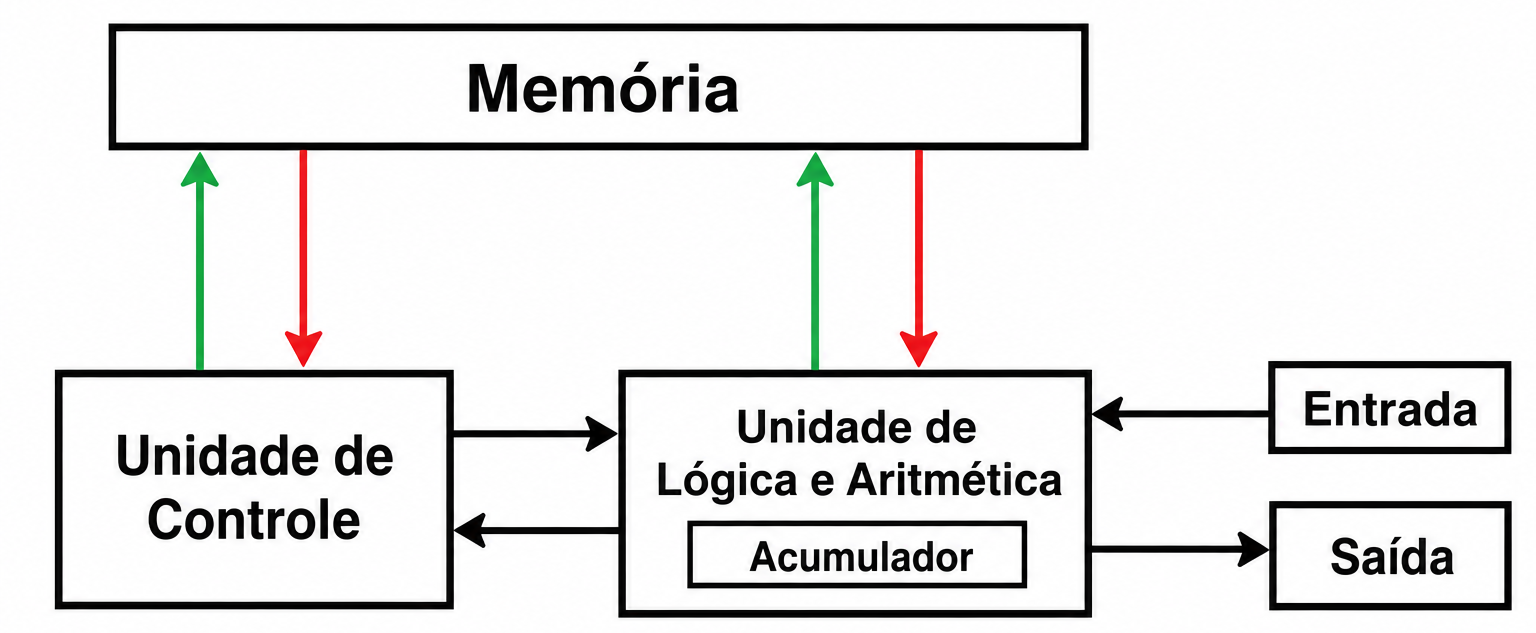
\includegraphics[width=0.8\linewidth]{Figuras/fig_diagrama_da_arquitetura.png}
    \label{fig:von_neumann}
    
    \vspace{0.1cm}
    \noindent\footnotesize{Fonte: Adaptado pelos autores (2026) de \citep{tanenbaum2013}.}
\end{figure}

Uma das principais limitações dessa arquitetura está na comunicação entre o processador e a memória. Como dados e instruções utilizam o mesmo canal, a transferência de informações pode não acompanhar a velocidade de processamento da 
CPU, fazendo com que ela precise aguardar os dados necessários. Essa limitação é conhecida como ``Gargalo de von Neumann'', expressão atribuída a John Backus durante sua palestra ao receber o Prêmio Turing, em 1977 \citep{couto2017}. 
O problema se tornou mais evidente com o aumento da velocidade dos processadores, que não foi acompanhado pelo mesmo crescimento na taxa de transferência entre a CPU e a memória \citep{couto2017}. Entre as soluções utilizadas estão a 
memória cache e a separação das caches de instruções e de dados, característica da arquitetura Harvard modificada \citep{couto2017}.

\subsection{Hierarquia de Memória e Princípio da Localidade}
\label{sec:hierarquia}

A fim de conciliar custo, capacidade e velocidade, os diferentes tipos de memória podem ser organizados de forma hierárquica. Essa hierarquia, tradicionalmente representada na forma de uma pirâmide que descreve seus níveis desde os mais 
rápidos e restritos até os de maior capacidade e menor velocidade, é composta por registradores, memória cache, memória principal e memória secundária (Figura~\ref{fig:hierarquia_memoria}).

\begin{figure}[ht]
    \centering
    \caption{Hierarquia de memória.}
    \label{fig:hierarquia_memoria}
    
    \vspace{0.2cm}
    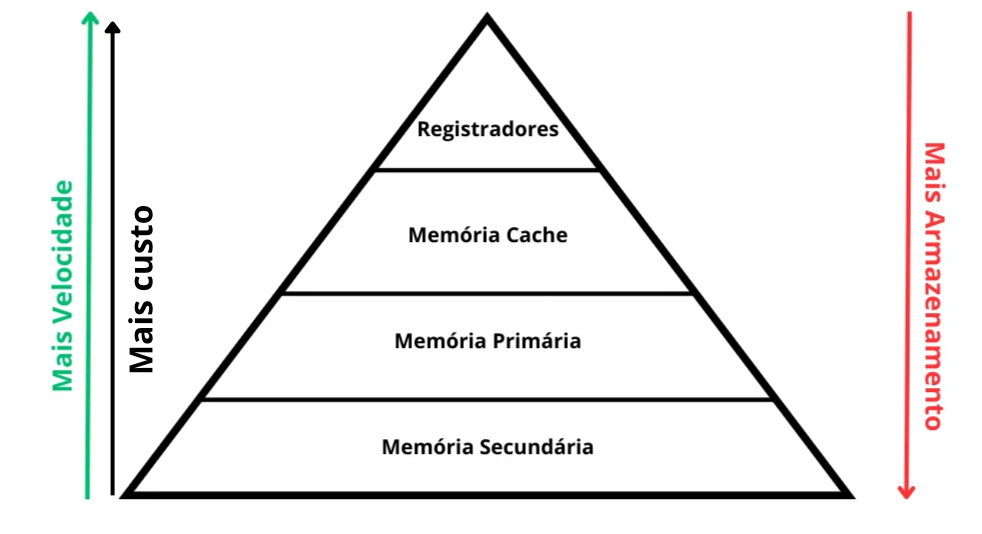
\includegraphics[width=0.8\linewidth]{Figuras/fig_hierarquia_memoria.png}
    
    \vspace{0.2cm}
    \noindent\footnotesize{Fonte: adaptado pelos autores (2026) de \citep{maues2025}.}
\end{figure}

As diversas camadas da hierarquia de memória apresentam as seguintes características funcionais e tecnológicas por \citep{maues2025}:

\begin{itemize}
    \item \textbf{Registradores:} localizados no topo da hierarquia, ficam no interior da CPU e representam o nível mais rápido, de menor latência e capacidade em comparação aos níveis inferiores, 
    e são responsáveis por armazenar operandos e instruções utilizados imediatamente pelo processador.
    \item \textbf{Memória Cache:} está no nível intermediário do diagrama, entre os registradores e a memória principal (RAM). A principal função da memória cache é armazenar dados e instruções mais frequentemente acessados para reduzir a 
    latência de acesso da CPU.
    \item \textbf{Memória Principal (RAM):} memória do tipo volátil (só guarda informações enquanto recebe energia), que armazena temporariamente as informações e dados enquanto programas e o sistema operacional estão em execução. 
    Em comparação às camadas acima, a memória principal é mais lenta, porém com capacidade substancialmente maior a um custo por bit mais baixo.
    \item \textbf{Memória Secundária:} são dispositivos de memória não voláteis, como discos rígidos (HDD) e unidades de estado sólido (SSD). Sendo o nível mais baixo da hierarquia, ela possui a maior 
    capacidade de armazenamento e menor custo por bit, consequentemente com a maior latência; esse tipo de memória tem como objetivo armazenar permanentemente dados, arquivos e o sistema operacional.
\end{itemize}

Um dos princípios fundamentais para que a hierarquia de memória funcione eficientemente é chamado de Princípio da Localidade de Referência. Esse princípio define que o processador tende a acessar 
sempre o mesmo conjunto de locais de memória. O Princípio da Localidade de Referência se divide em dois tipos:

\begin{itemize}
    \item \textbf{Localidade Temporal:} a Localidade Temporal diz que, se um dado ou instrução foi acessado recentemente, tem uma grande chance de ser requisitado novamente em um curto intervalo de 
    tempo pelo processador. Alguns exemplos são funções, métodos, laços de repetição, contadores e variáveis frequentemente modificadas \citep{ferreira2015}.
    \item \textbf{Localidade Espacial:} a Localidade Espacial afirma que, se um endereço de memória foi recentemente acessado pelo processador, tem uma grande chance de blocos seguintes ou próximos 
    a essa localização também serem acessados em seguida. Isso ocorre, por exemplo, com as partes procedurais e sequenciais de um programa, além de estruturas de dados como vetores, matrizes e listas \citep{ferreira2015}.
\end{itemize}

\subsection{Funcionamento e Estratégias da Memória Cache}
\label{sec:amat}

Sem a memória cache, cada ciclo de instrução requer, no mínimo, um acesso à memória principal. Como a DRAM é substancialmente mais lenta do que a execução da instrução, o processador passa bastante tempo ocioso 
\citep{ferreira2015}. A cache diminui o gargalo causado por esse descompasso a partir do armazenamento de cópias das instruções e dos dados mais utilizados \citep{stallings2010, ferreira2015}. Quando a CPU requisita 
uma palavra, ocorre um acerto de cache (\textit{cache hit}): caso ela esteja contida em alguma linha da cache, será entregue ao processador em um tempo $T_{acerto}$. Caso contrário, ocorre uma falha (\textit{cache miss}), 
e a palavra deve ser buscada em um nível inferior, busca esta que incide em uma penalidade $P_{falha}$, a qual depende da latência da DRAM e também do tráfego do barramento. Durante esta operação, são transferidas não só a palavra 
requisitada, mas um bloco de palavras adjacentes para diminuir a possibilidade de futuros \textit{misses}, levando em conta a localidade espacial \citep{stallings2010, ferreira2015}.

O impacto na memória cache pode ser mensurado pelo tempo médio de acesso à memória (AMAT) que, com base no modelo de dois níveis de \citep{stallings2010}, é dado por:
\begin{equation}\label{eq:amat}
T_{med} = T_{acerto} + (1 - h) \times P_{falha}
\end{equation}
em que $h$ é a taxa de acerto e $(1 - h)$ é a taxa de falhas. Por exemplo: utilizando valores hipotéticos como $T_{acerto} = 5\text{ ns}$ (ordem de grandeza de uma cache L2), $P_{falha} = 60\text{ ns}$ e $h = 0,95$, tem-se $T_{med} = 5 + 0,05 \times 60 = 8\text{ ns}$. 
Isto significa que, embora a penalidade de falha seja doze vezes o tempo de acerto, a média fica próxima à ordem de grandeza do tempo de acesso à memória cache; ainda assim, as falhas, mesmo ocorrendo em apenas 5\% dos acessos, respondem por 3 dos 8 ns (37,5\%).

Vários desses aspectos são considerados em projetos de cache, que combinam algumas estratégias. A hierarquia multinível divide a cache em níveis L1, L2 e L3, onde a L1 é a mais baixa e rápida nessa sub-hierarquia e se localiza internamente 
ao processador; a L2 é intermediária; e a L3 é a última barreira antes da DRAM, sendo compartilhada entre os núcleos (enquanto a L1 e L2 são exclusivas de cada núcleo). Assim como na hierarquia de memória, quanto mais baixo for o nível de cache, maior será a capacidade 
e menor a velocidade de operação; consequentemente, quanto mais próximo do processador for o nível, maior será a velocidade e menor a capacidade da memória \citep{stallings2010, ferreira2015}. Além disso, a cache L1 pode ser dividida em instruções (L1I) e dados (L1D), 
o que evita a concorrência entre a busca de instruções e a unidade de execução no pipeline. Essa divisão concretiza a arquitetura Harvard modificada descrita na Seção~\ref{sec:metodologia}; no entanto, a cache unificada tende a apresentar maior taxa de acerto para o mesmo 
tamanho de palavras \citep{stallings2010}. Outra estratégia de atenuação do gargalo é o mapeamento de endereços: que pode ser direto, associando cada bloco a uma única linha (abordagem simples e barata, mas sujeita a faltas por conflito); já o mapeamento totalmente associativo 
permite qualquer linha, não possui problema de conflito, mas exige comparar as etiquetas de todas elas de forma exaustiva; e o associativo por conjuntos de $k$ vias oferece um bom equilíbrio entre a simplicidade do mapeamento direto e a flexibilidade do associativo \citep{stallings2010}. 
Na política de escrita \textit{write-through}, a palavra é gravada direto na DRAM a cada vez que ocorre uma escrita, mantendo a consistência de ambos os níveis, contudo podendo saturar o barramento a depender do tráfego gerado; já o \textit{write-back} grava a palavra diretamente na memória 
cache, marca a linha com um bit de modificação (\textit{dirty bit}) e atualiza a DRAM somente quando o bloco é descartado \citep{stallings2010}. \citep{ferreira2015} relata ganhos de até 15 por cento em processadores Cyrix e de cerca de 30 por cento em processadores IBM com a política de 
\textit{write-back}. Por fim, quando o conjunto está cheio na memória cache, algoritmos como LRU (que descarta o bloco menos recentemente utilizado, para preservar a localidade temporal), FIFO ou aleatório escolhem o bloco a ser substituído \citep{stallings2010}.

\subsection{Estratégias no Armazenamento Secundário} 
\label{sec:secundario}
Em geral, o armazenamento secundário apresenta latência bem superior à das memórias voláteis, por depender de meios físicos para a gravação de dados \citep{oliveira2019, stallings2010}. Os HDDs são os principais armazenadores de longo prazo por terem um baixo custo e grande capacidade. 
Porém, para ler um dado, o braço de leitura precisa ser posicionado para pesquisa (\textit{seek time}), que varia entre 4 e 10 ms, e o disco deve girar até que o setor seja acessado (latência rotacional), que varia entre 3 e 7 ms \citep{santos2015}. Essa característica torna o acesso custoso e 
gera um tempo mais lento do que o acesso à DRAM. Assim, uma das grandes dificuldades de projeto é lidar com E/S.

Uma estratégia é o uso de memória virtual: a partir da necessidade de mais memória RAM do que a disponível por parte dos programas, o sistema operacional divide o espaço de endereçamento em páginas de tamanho fixo. A página é carregada a partir do disco, conforme necessário, para uma área chamada 
\textit{swap} \citep{souza2023}. Esse processo corre o risco de gerar o \textit{thrashing}, que ocorre quando o conjunto de trabalho (\textit{working set}) é maior que a RAM e, consequentemente, a maior parte dos ciclos é consumida na transferência de páginas entre o disco e a memória, o que prejudica 
o sistema \citep{souza2023}. 

Os SSDs são mais rápidos que os HDDs pois utilizam memória NAND \textit{flash}. Porém, não são vistos para substituir os HDDs para conjuntos massivos de dados, pois possuem custo mais alto por gigabyte, além de uma capacidade menor. Uma alternativa é utilizar o SSD como uma cache transparente dos dados 
mais acessados do HDD \citep{santos2015}. No Linux, existem soluções como \textit{BCache} e \textit{DMCache}. O \textit{BCache} trabalha na camada de blocos, independente do sistema de arquivos, e possui a vantagem de permitir acesso aleatório e ignorar solicitações estritamente sequenciais. O \textit{DMCache} 
utiliza o \textit{device-mapper} e exige partições dedicadas; além disso, permite três modos de escrita: \textit{write-back} (apenas na cache), \textit{write-through} (na cache e no dispositivo subjacente ao mesmo tempo) e \textit{write-around} (diretamente no dispositivo subjacente) \citep{santos2015}. A Figura
~\ref{tab:estrategias_mitigacao} compara as estratégias de armazenamento secundário com as de cache.

\begin{figure*}[ht]
\caption{Estratégias de mitigação do Gargalo de von Neumann.}
\centering
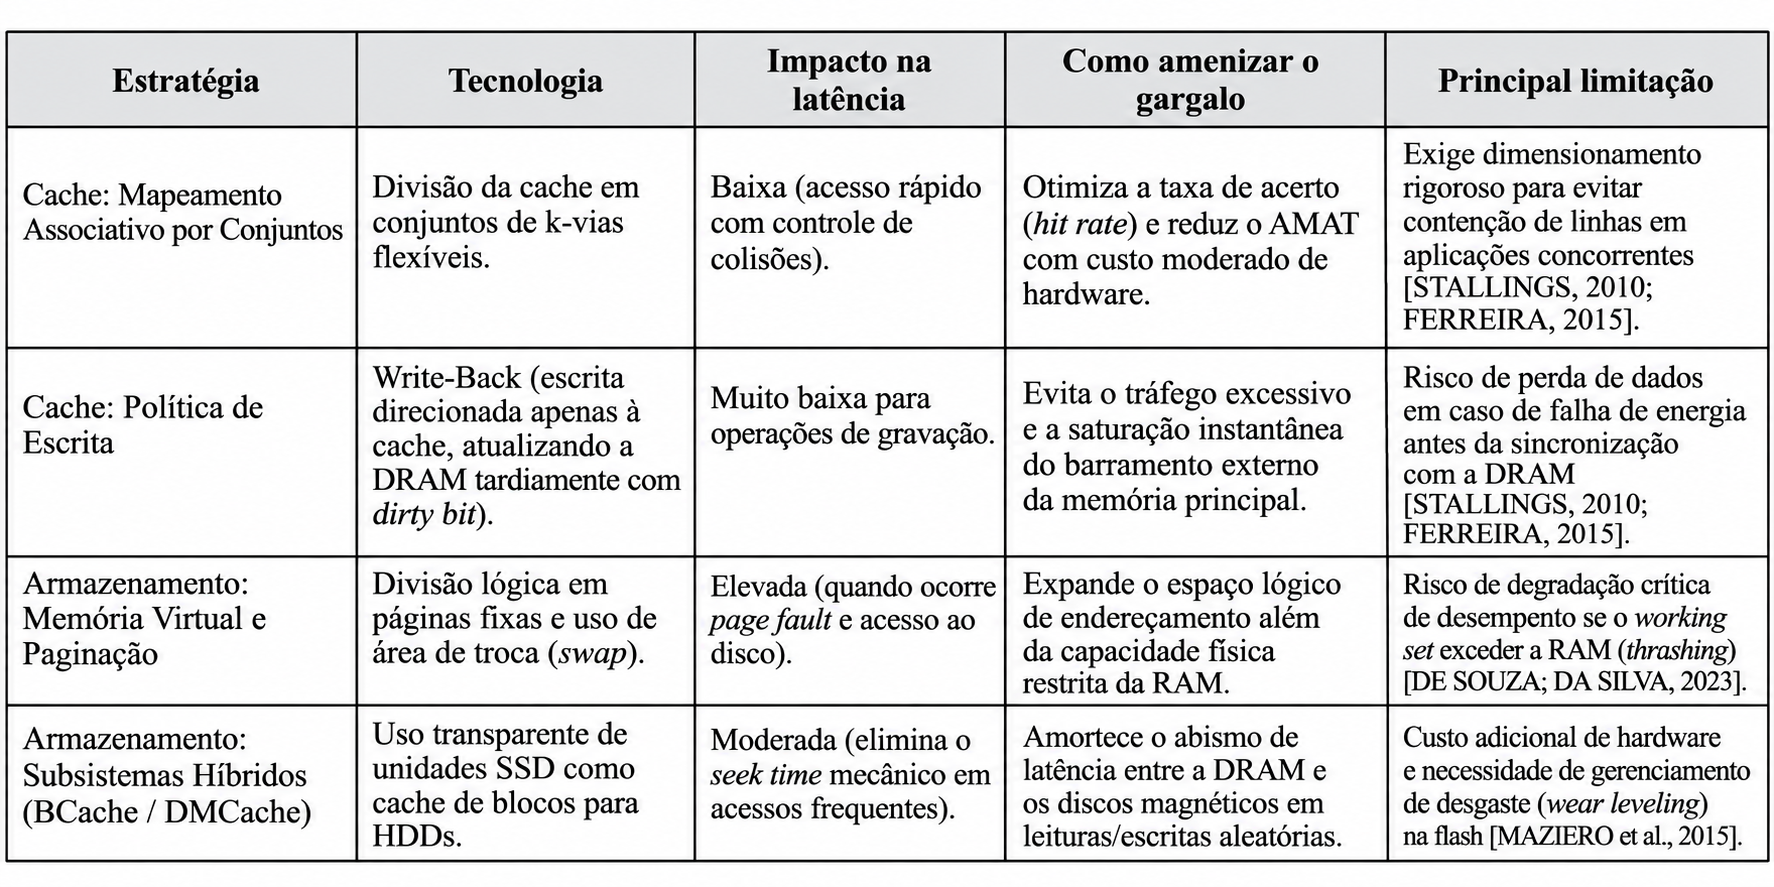
\includegraphics[width=\textwidth]{Tabelas/tab_estrategias_mitigacao.png}
\label{tab:estrategias_mitigacao}
\footnotesize{\textit{Fonte:} Elaborado pelos autores (2026), com base em \citep{stallings2010, ferreira2015, souza2023, santos2015}.}
\end{figure*}

\section{Análise Crítica e Gargalos Arquiteturais}

\subsection{O Descompasso Físico e os Limites da Escalabilidade} \label{sec:limitacoes}
Com o avanço das tecnologias de processadores, as memórias principais não acompanharam este avanço. Isto resulta em casos nos quais a CPU entra em modo de espera (wait time) para aguardar a chegada dos dados \citep{stallings2010, tanenbaum2013}. O problema ocorre devido ao fato de que a DRAM armazena informações 
em capacitores, que ao receberem um bit, perdem carga ao longo do tempo, exigindo ciclos periódicos de atualização (\textit{refresh}). Já a SRAM da cache utiliza flip-flop para armazenamento, não precisa realizar refresh, porém requer mais transistores para armazenar um bit, resultando em maior custo de implementação 
e menor densidade de integração \citep{stallings2010}. Desta forma, a memória cache é rápida, porém com pequena capacidade e alto custo, sendo a memória principal de maior capacidade, porém mais lenta. (Figura~\ref{tab:tradeoffs_hierarquia}).

O aumento da frequência de operação também fez surgir limites físicos: a partir de 2001, o aquecimento causado pela redução espacial dos transistores não podia ser dissipado utilizando-se refrigeração convencional. Isto fez com que o aumento do clock se tornasse difícil, o que levou os fabricantes a resolverem este impasse 
utilizando-se de processadores multicore \citep{ferreira2015}. Com vários núcleos, o barramento tende a se tornar um ponto de contenção arquitetural. Para contornar essa situação, foi utilizada uma cache L3 compartilhada entre todos os núcleos (microarquitetura Nehalem). Esta cache atua inclusivamente sobre as caches L1 e L2 de 
cada núcleo, e evita que cada núcleo verifique a cache privada dos outros núcleos, o que aumenta consideravelmente o rendimento do sistema como um todo \citep{ferreira2015}.

\subsection{Síntese dos Trade-Offs}
\label{sec:analise}

A Figura~\ref{tab:tradeoffs_hierarquia} apresenta uma síntese comparativa dos níveis que compõem a hierarquia de memória e destaca suas respectivas ordens de grandeza típicas de latência, as capacidades ilustrativas e os principais compromissos de projeto associados a cada tecnologia.

\begin{figure*}[!ht]
\caption{Tabela comparativa dos níveis da hierarquia de memória e trade-offs arquiteturais.}
\centering
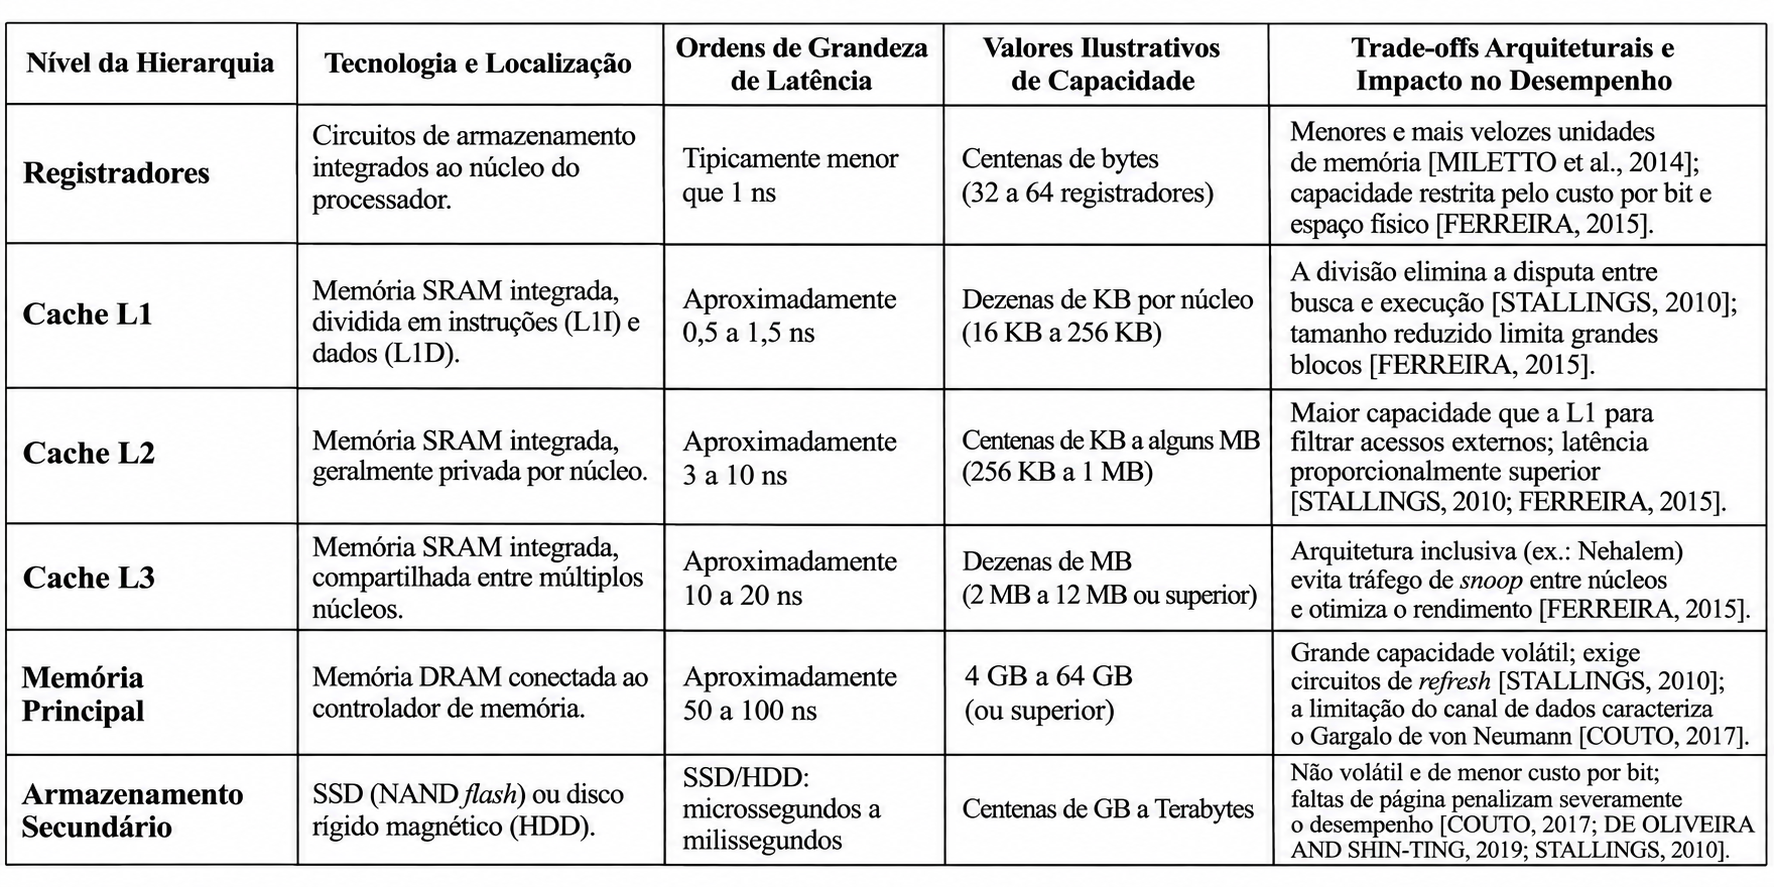
\includegraphics[width=\textwidth]{Tabelas/tab_tradeoffs_hierarquia.png}
\label{tab:tradeoffs_hierarquia}
\footnotesize{Fonte: Elaborado pelos autores (2026) com base em \citep{couto2017, ferreira2015, hennessy2017, miletto2014, oliveira2019, stallings2010}. A capacidade das memórias e as ordens de grandeza de latência por nível são baseadas em \citep{hennessy2017}.}
\end{figure*}

Em síntese, a Figura~\ref{tab:tradeoffs_hierarquia} evidencia os \textit{trade-offs} centrais da hierarquia de memória: o alto desempenho e a baixa latência dos registradores e memória cache têm como contrapartida a elevada capacidade e persistência de dados dos níveis mais baixos, ou seja, DRAM e memória secundária. 
Logo, podemos concluir que, no geral, quanto maior a capacidade de um nível, menor é sua velocidade de acesso. Assim, o desempenho computacional global depende diretamente da eficiência com que o gargalo de von Neumann é mitigado ao longo de todos os níveis da hierarquia de memória.

\section{Considerações Finais}
\label{sec:conclusao}

Este estudo discutiu as principais estratégias para diminuir o Gargalo de von Neumann em cada nível da hierarquia de memória. A desproporção de velocidades entre a CPU e a latência da memória RAM é agravada pela barreira térmica de \textit{clock} e a contenção de barramentos em sistemas \textit{multicore} 
~\citep{ferreira2015, tanenbaum2013}. As soluções encontradas na literatura para contornar este gargalo consistem em utilizar caches hierárquicos, que exploram os princípios de localidade de dados e instruções para reduzir o tempo médio de acesso. Políticas de escrita como o \textit{Write-Back}, \textit{Write-through} e 
\textit{Write-Around} nas memórias cache ~\citep{stallings2010, ferreira2015}, bem como na utilização de SSDs e subsistemas de cache de bloco no armazenamento secundário para reduzir a diferença relativa de latência dos HDDs ~\citep{santos2015}. Contudo, é importante ressaltar que este gargalo não foi eliminado, mas apenas 
reduzido pelas estratégias descritas, visto que ainda existirá um certo atraso nas interações entre a CPU e os diversos tipos de memórias, por menor que seja.

As tendências futuras na computação, impulsionadas principalmente pela inteligência artificial, demonstram as limitações atuais destas estratégias. Os bilhões de pesos de um modelo são constantemente carregados da memória, além disso, somado ao tráfego extenso de informações e instruções, a maior parte da energia elétrica é 
consumida nessa transferência de dados, com o cálculo representando apenas cerca de 10\% da carga, segundo pesquisadores da IBM \citep{hess2025}. Novas soluções estão surgindo para contornar essa situação: entre elas está a computação em memória, onde os pesos do modelo são guardados na resistividade do material por meio da 
Memória de Mudança de Fase (\textit{Phase Change Memory} - PCM), com o intuito de minimizar transferência de dados. Porém, devido à baixa durabilidade da PCM, essa abordagem limita sua aplicação em modelos já treinados em GPUs. Outras inovações incluem a computação próxima à memória, como o processador IBM NorthPole, onde cada 
núcleo do processador possui sua própria memória SRAM integrada. Outro exemplo é a óptica co-embalada, na qual a largura de banda da fibra óptica é levada até a borda do chip \citep{hess2025}. 

Enquanto a arquitetura de von Neumann continuar sendo essencial para a computação geral e para operações precisas, tendências indicam a chegada de sistemas híbridos que combinem arquiteturas de von Neumann e não von Neumann \citep{hess2025}.

\begin{declarations}

\begin{contributions}
Ambos os autores, juntos, contribuíram para a idealização, realização da pesquisa bibliográfica, redação e revisão de toda a parte estrutural desse estudo como um todo, além da elaboração e adaptação dos diagramas e tabelas a partir da síntese dos conteúdos achados sobre o assunto. Quanto às contribuições individuais, 
enquanto um ficou responsável pela pesquisa e organização das estratégias de mitigação do Gargalo de von Neumann na memória cache, o outro atuou nas análises do armazenamento secundário. O manuscrito final foi lido e aprovado por ambos os autores.
\end{contributions}

\begin{interests}
Os autores declaram que não têm nenhum conflito de interesses. 
\end{interests}

\begin{materials}
Os dados e outros materiais criados e/ou usados nesta revisão da literatura 
serão disponibilizados mediante solicitação. 
\end{materials}

\begin{aitools}
O texto foi redigido pelos autores. Ferramentas de inteligência artificial generativa 
— especificamente Claude Sonnet 5.5 (Anthropic), ChatGPT na versão GPT-6 (OpenAI) e Gemini (Google) —  
foram utilizadas exclusivamente para checagem ortográfica e gramatical do documento, além de auxiliar na 
estruturação do código \LaTeX, conforme definido nas diretrizes da revista RICA.
\end{aitools}

\begin{furtherinformation}
Por ser um estudo de revisão bibliográfica, não houve coleta de dados primários, nem experimentos com seres 
humanos ou animais, logo não houve necessidade de aprovação da pesquisa por um comitê de ética.
\end{furtherinformation}

\end{declarations}

\bibliographystyle{apalike-sol}
\bibliography{refs}

\end{document}

